%==============================================================================
%== template for LATEX poster =================================================
%==============================================================================
%
%--A0 beamer slide-------------------------------------------------------------
\documentclass[final]{beamer}
\usepackage[orientation=portrait,size=a1,
            scale=.85         % font scale factor
           ]{beamerposter}
\setlength{\paperwidth}{33.1in}
\setlength{\paperheight}{23.4in}
%\setlength{\paperwidth}{60in}
%\setlength{\paperheight}{36in}
           
\geometry{
  hmargin=2.5cm, % little modification of margins
}

\providecommand{\tightlist}{%
  \setlength{\itemsep}{0pt}\setlength{\parskip}{0pt}}


%
\usepackage[utf8]{inputenc}

\linespread{1.15}
%
%==The poster style============================================================
\usetheme{sharelatex}

%==Title, date and authors of the poster=======================================
\title
[International Digital Curation Conference. Edinburgh, Scotland. February
20-23, 2017.] % Conference
{ % Poster title
Community Engagement for Developing the Principles and Practices of
Agile Data Curation
}

\author{ % Authors
Karl Benedict\inst{1} \and W. Christopher Lenhardt\inst{2} \and Joshua Young\inst{3}}

\institute{
\inst{1} University of New Mexico
\inst{2} Renaissance Computing Institute
\inst{3} University Corporation for Atmospheric Research
}


\date{December 15, 2016}



\begin{document}
\begin{frame}[t]
%==============================================================================
\begin{multicols}{2}

%--abstract-------------------------------------------------------------

\subsection{Abstract}

The combination of increasing demands for more systematic data
management planning in support of effective in-project data management,
research data sharing, and long-term preservation of discovery and
access; increasing volumes of data being created and used in research;
and research support budgets that aren't increasing in proportion to
these demands is creating a situation in which greater efficiencies and
product-centered research data management workflows and processes are
needed. Taking inspiration from the principles and practices of agile
software development, the presenters of this poster are working towards
the development of three sets of interdependent products. First, a set
of \emph{core principles} that have broad support within the community
will be identified and/or developed from existing statements of
principles; solicited from the broad community of research data
creators, curators, and users; and derived from implicit principles
exemplified by specific research data projects that have achieved
notable success in enabling efficient use, preservation, discovery and
reuse. Second, building upon the case studies identified and reviewed as
part of the aforementioned process of identifying core data management
principles, additional case studies are being sought that demonstrate
effective research data management practices that are aligned with the
identified principles and have resulted in well structured, effectively
preserved, and documented data sets that are well-positioned for
discovery and reuse by diverse users. And third, the development of a
collection of research data curation design patterns that can provide
structured guidance to researchers and data curators in developing
workflows that deliver incremental increases in research data value
through time, both to the researchers who are creating and using data
for the first time and for future users of those data. This progression
from values and principles through current exemplars to documented
recommended practices \emph{that are of sufficient specificity to be
actionable} is anticipated to produce the theoretical \emph{and}
operational foundation needed for more efficient development and
delivery of research data value. This greater efficiency has the
potential to allow for the continued growth of the volume, diversity,
and rate of creation within limited resources, while also enabling more
effective collaboration among increasingly large and diverse research
teams.

%--End of abstract------------------------------------------------------




%==============================================================================
%==The poster content==========================================================
%==============================================================================

\section{Introduction}\label{introduction}

Thus far the focus of the project's work has been on developing a
framework within which the team can discuss the concept of \emph{agile
data curation} with the community, and iteratively evolving that
framework through a series of meeting sessions, workshops and
presentations that have been given at multiple venues including the
American Geophysical Union (2014, 2015), Federation of Earth Science
Information Partners Meeting (2016), Research Data Alliance (2014, 2015,
2016), and SciDataCon (2016). In these various activities the team has
worked on communicating the conceptual framework for our vision of agile
data curation, presented a variety of initial values and principles
derived from those defined in the \emph{Manifesto for Agile Software
Development} (Beck et al., 2001), and solicited the presentation of data
management projects that exemplify (either intentionally or
unintentionally) these principles. The purpose of the presentation below
is to expand this discussion to a broader international and disciplinary
audience in support of moving forward with soliciting input into the
definition of a set of shared values and principles, and collection of
illustrative case studies in support of the development of design
patterns that may be applied to diverse data curation problems.

\section{Values and Principles}\label{values-and-principles}

At the foundation of a conceptual mapping between \emph{Agile Software
Development} and \emph{Agile Data Curation} the primary focus is not on
the various agile software development methodologies that have been
developed, but instead on the underlying values and principles (Beck et
al., 2001) that have been identified as a foundation for multiple
methodologies identified as \emph{agile}. Below are some initial
\emph{agile data curation} values and principles that the authors have
developed as a point of departure for a community discussion.

\subsection{Mapping of Agile Software Development Values into Data
Curation}\label{mapping-of-agile-software-development-values-into-data-curation}

\textbf{Agile Software Development}

\begin{itemize}
\tightlist
\item
  \emph{Individuals and interactions} over processes and tools
\item
  \emph{Working software} over comprehensive documentation
\item
  \emph{Customer collaboration} over contract negotiation
\item
  \emph{Responding to change} over following a
  plan{[}\^{}agilePrinciples{]}
\end{itemize}

\textbf{Agile Data Curation}

\begin{itemize}
\tightlist
\item
  \emph{Individuals and interactions} over processes and tools
\item
  \emph{Discoverable, understandable and usable data} over comprehensive
  documentation
\item
  \emph{User collaboration} over contract negotiation
\item
  \emph{Responding to change} over following a plan
\end{itemize}

\subsection{Mapping of Agile Software Development Principles into Data
Curation}\label{principles}

\textbf{Agile Software Development Principles}

\begin{itemize}
\tightlist
\item
  Our highest priority is to satisfy the customer through early and
  continuous delivery of valuable software.
\item
  Welcome changing requirements, even late in development. Agile
  processes harness change for the customer's competitive advantage.
\item
  Deliver working software frequently, from a couple of weeks to a
  couple of months, with a preference to the shorter timescale.
\item
  Business people and developers must work together daily throughout the
  project.
\item
  Build projects around motivated individuals. Give them the environment
  and support they need, and trust them to get the job done.
\item
  The most efficient and effective method of conveying information to
  and within a development team is face-to-face conversation.
\item
  Working software is the primary measure of progress.
\item
  Agile processes promote sustainable development. The sponsors,
  developers, and users should be able to maintain a constant pace
  indefinitely.
\item
  Continuous attention to technical excellence and good design enhances
  agility.
\item
  Simplicity--the art of maximizing the amount of work not done--is
  essential.
\item
  The best architectures, requirements, and designs emerge from
  self-organizing teams. At regular intervals, the team reflects on how
  to become more effective, then tunes and adjusts its behavior
  accordingly.
\end{itemize}

\textbf{Agile Data Curation Principles}

\begin{itemize}
\tightlist
\item
  Maximize the impact of research data through accelerated capacity for
  discovery, access and use of valuable data
\item
  Expect unanticipated needs for and uses of research data (and
  documentation) and develop flexible systems to support new uses and
  users without significant modifications
\item
  Facilitate automated interaction with data and metadata assets through
  well documented public web services that enable disintermediated use
  and reuse of research data
\item
  Data creators and data curators should work closely throughout
  planning, research and preservation activities to ensure the most
  efficient and streamlined process
\item
  Identify key individuals in a data curation project that have the
  requisite knowledge and motivation to do the job and get out of their
  way
\item
  Identify the most effective method(s) for maintaining close
  communication and \emph{use} them
\item
  Delivery, access, use and citation of research data are the primary
  measures of success
\item
  Design principles that enable steady delivery of incremental
  improvements to research data discovery, access and use should be
  consistent with a sustainable level of effort and funding from
  sponsors, data creators and curators, and users
\item
  Continuous attention to technical excellence and good design enhances
  agility
\item
  Start with the basics and only make systems more complex as needed,
  while maintaining a low bar to entry
\item
  Continuously work to develop and evolve a community of data providers,
  curators and users that all participate in the ongoing evolution of
  the research data systems that they interact with
\end{itemize}

\section{Case Studies into Design
Patterns}\label{case-studies-into-design-patterns}

Below is an illustration of an initial set of existing design patterns
from a software development context that can provide elements for
addressing elements of a combination of research and data lifecycles,
the OAIS archival framework, and the capabilities of a specific data
management, discovery and access platform (Benedict, 2017); the
Geographic Storage, Transformation and Retrieval Engine - GSToRE -
(bottom - Earth Data Analysis Center (EDAC), 2016) developed in support
of a specific set of research and application requirements

\begin{figure}[htbp]
\centering
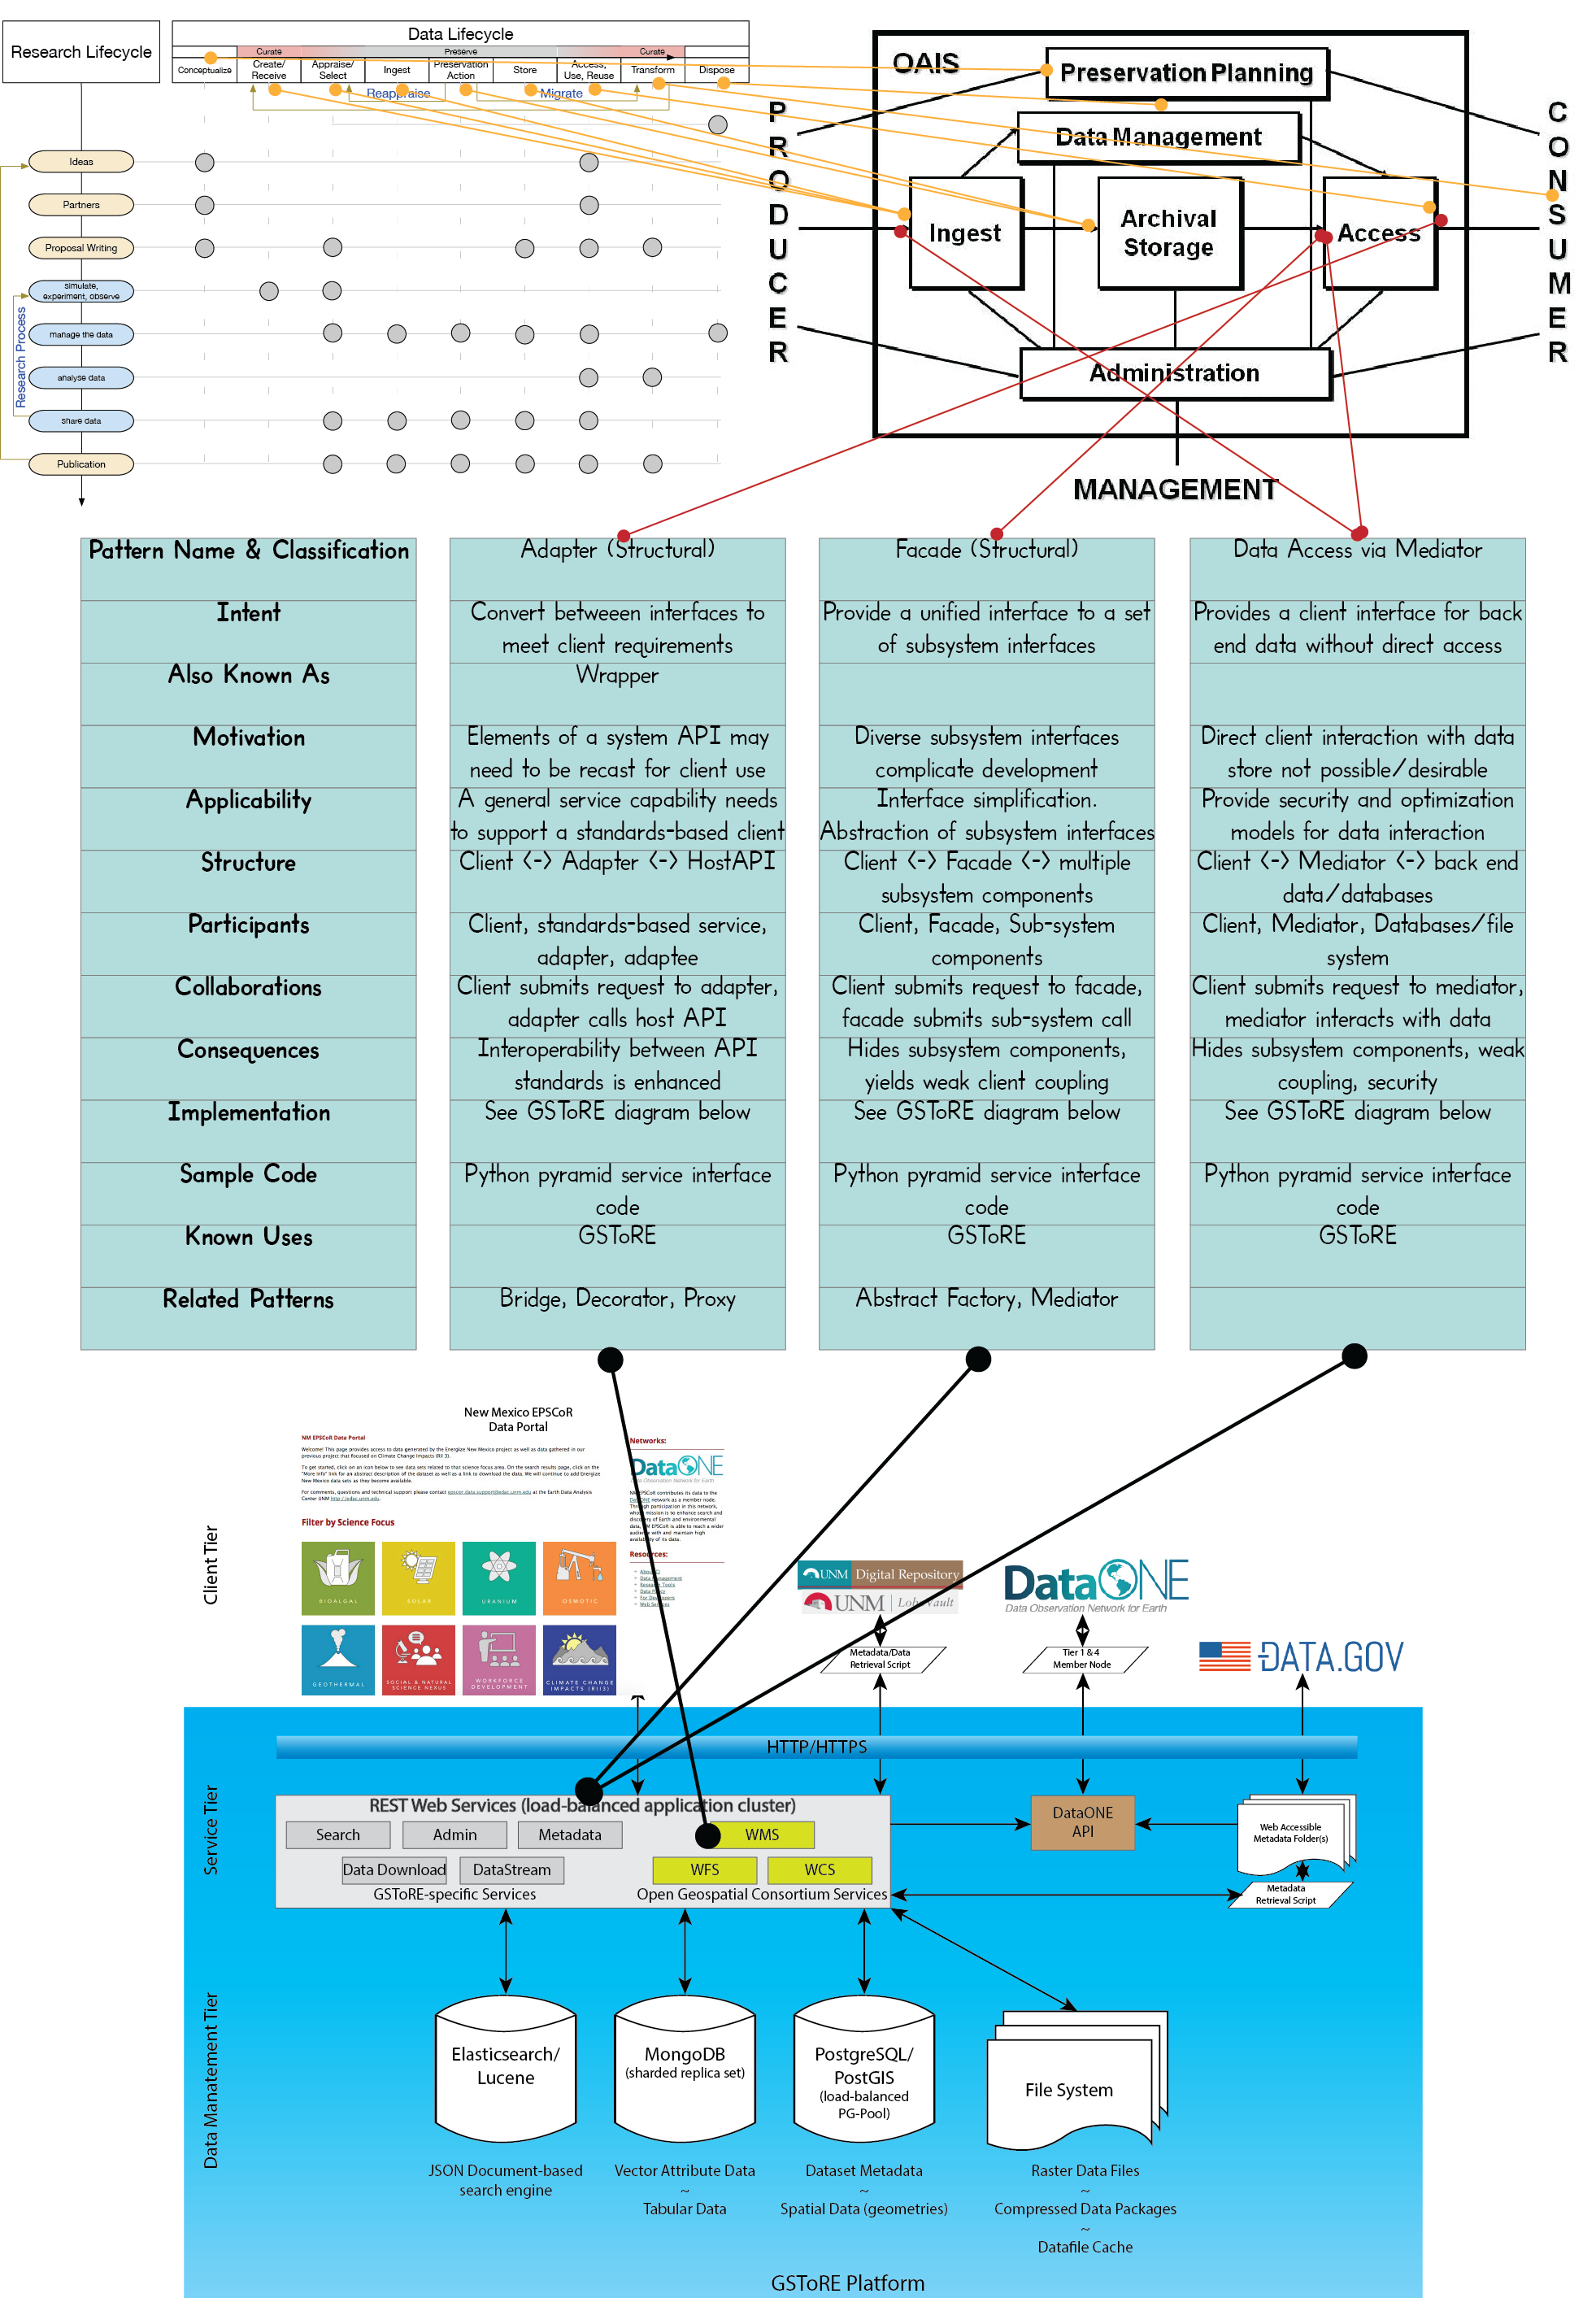
\includegraphics[width=8.00000in]{Composite-DesignPatternMapping.png}
\caption{Mapping of the GSToRE Platform's Capabilities into a Set of
Design Patterns (middle - Gamma et al., 1995, pp 135, 185; Schwinn and
Schelp, 2005, pp 476) and corresponding linkages between the OAIS
Framework (upper right - Consultative Committee for Space Data Systems
(CCSDS), 2012; International Organization for Standardization (ISO),
2012; Lavoie, 2014) and an Illustration (upper left) of the Intersection
of the Research Lifecycle (JISC, 2014) and Data Curation Lifecycle
Actions (Digital Curation Centre (DCC), nd)}
\end{figure}

\subsection{Bibliography}\label{bibliography}

~

\hypertarget{refs}{}
\hypertarget{ref-beckux5fmanifestoux5f2001}{}
Beck, K., Beedle, M., van Bennekum, A., Cockburn, A., Cunningham, W.,
Fowler, M., Grenning, J., Highsmith, J., Hunt, A., Jeffries, R., Kern,
J., Marick, B., Martin, R.C., Mellor, S., Schwaber, K., Sutherland, J.,
Thomas, D., 2001. Manifesto for Agile Software Development.

\hypertarget{ref-benedictux5fgeographicux5f2017}{}
Benedict, K., 2017. The Geographic Storage, Transformation and Retrieval
Engine (GSToRE): A Platform for Active Data Access and Publication as a
Complement to Dedicated Long-Term Preservation System, in: Curating
Research Data. Volume Two, A Handbook of Current Practice. Association
of College and Research Libraries, Chicago, IL, pp. 207--209.

\hypertarget{ref-bookux5freferenceux5f2012}{}
Consultative Committee for Space Data Systems (CCSDS), 2012. Reference
Model for an Open Archival Information System (OAIS) (No. CCSDS
650.0-M-2). Consultative Committee for Space Data Systems (CCSDS).

\hypertarget{ref-digitalux5fcurationux5fcentreux5fdccux5fdccux5fnd}{}
Digital Curation Centre (DCC), nd. DCC Curation Lifecycle Model
\textbar{} Digital Curation Centre.

\hypertarget{ref-ux5fgstoreux5f2016}{}
Earth Data Analysis Center (EDAC), 2016. GStore V3 API.

\hypertarget{ref-gammaux5fdesignux5f1995}{}
Gamma, E., Helm, R., Johnson, R., Vlissides, J., 1995. Design patterns:
Elements of reusable object-oriented software, Addison-wesley
professional computing series; addison-wesley professional computing
series. Addison-Wesley, Reading, Mass.

\hypertarget{ref-ux5fisoux5f2012}{}
International Organization for Standardization (ISO), 2012. ISO
14721:2012 - Space data and information transfer systems -- Open
archival information system (OAIS) -- Reference model. ISO.

\hypertarget{ref-ux5fhowux5f2014}{}
JISC, 2014. How Jisc is helping researchers : Jisc.

\hypertarget{ref-oclcux5fopenux5f2014}{}
Lavoie, B., 2014. The Open Archival Information System (OAIS) Reference
Model: Introductory Guide (2nd Edition). Digital Preservation Coalition.

\hypertarget{ref-schwinnux5fdesignux5f2005}{}
Schwinn, A., Schelp, J., 2005. Design patterns for data integration.
Journal of Enterprise Information Management 18, 471--482.
doi:\href{https://doi.org/10.1108/17410390510609617}{10.1108/17410390510609617}

%==============================================================================
%==End of content==============================================================
%==============================================================================

%--Acknowledgements-------------------------------------------------------------

\subsection{Acknowledgements}

This work has been partially supported through funding from the National
Science Foundation (\#IIA-1301346)

%--End of Acknowledgements------------------------------------------------------


%--References------------------------------------------------------------------



%--End of references-----------------------------------------------------------

\end{multicols}

%==============================================================================
\end{frame}
\end{document}
